\section{Durchführung}
\label{sec:Durchführung}
Die verscheidenen Wärmeleitfähigkeiten werden mithilfe des folgenden Versuchsaufbaus \ref{fig:aufbau}
untersucht. Die Thermoelemente haben jeweils den Abstand \SI{30}{\milli\meter}.
\begin{figure}
    \centering
    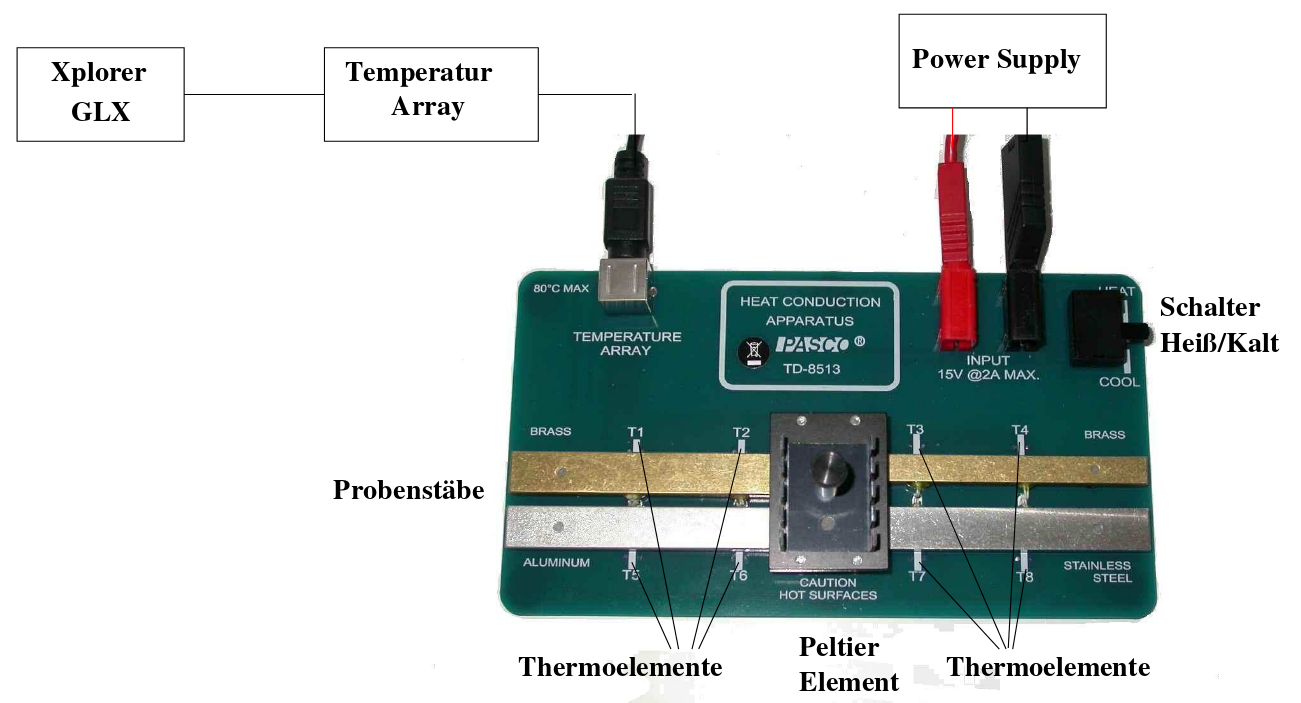
\includegraphics[width=\textwidth]{content/aufbau.png}
    \caption{Versuchsaufbau.}
    \label{fig:aufbau}
\end{figure}
Dabei heizt das Peltierelement die vier Metallstäbe simultan und die Temperatur wird an 8
verschiedenen Messpunkten, je zwei pro Stab, mithilfe vom Thermoelementen gemessen. Die
Messwerte werden über ein Temperature Array mit einem Datenlogger aufgezeichnet.
%
\subsection{Statische Methode}
\label{sec:statische Methode}
Das Peltierelement wird mit $U_\text{P}=\SI{5}{\volt}$ betrieben.
Die vier Eisenstäbe werden eine halbe Stunde lang erheitzt.
An den acht Thermoelementen wird die Temperatur gemessen und der jeweilige Wert alle 5 Sekunden gespeichert.
Anschließend werden die Stäbe durch das Peltierelement gekühlt.
%
\subsection{Dynamische Methode}
\label{sec:dynamische Methode}
Bei der dynamischen Methode, auch Angström-Verfahren, wird im Gegensatz zur statischen Methode nicht kontinuierlich, 
sondern periodisch mit $U_\text{P}=\SI{8}{\volt}$ geheizt und gekühlt. 
Der Datenlogger wird außerdem auf eine Abtastperiode von $\SI{2}{\second}$ gestellt.
Es ergibt sich innerhalb des Materials eine Temperaturwelle der Form \eqref{eqn:thermowelle}.
In der ersten Messung wurden zehn Perioden mit einer Periodendauer von $\SI{80}{\second}$ aufgezeichnet, 
in der zweiten Messung wurde etwa eine Stunde lang mit eine Periodendauer von $\SI{400}{\second}$ gemessen.
